\documentclass[12pt, titlepage]{article}

\usepackage{booktabs}
\usepackage{tabularx}
\usepackage{hyperref}
\hypersetup{
    colorlinks,
    citecolor=black,
    filecolor=black,
    linkcolor=red,
    urlcolor=blue
}
\usepackage[round]{natbib}
\usepackage[left=1in, right=1in, top=1in, bottom=1in]{geometry}
\usepackage{graphicx}
\usepackage{hhline}
\usepackage{enumerate}
\usepackage{enumitem}
%\usepackage{biblatex}
\usepackage{xcolor}
\usepackage[normalem]{ulem}

\title{SE 3XA3: Software Requirements Specification\\\textcolor{red}{Random Flag Generator \sout{FlagGenerator}}}

\author{Team \#2, Team Jakriel
        \\ Akram Hannoufa, hannoufa
        \\ Ganghoon (James) Park, parkg10
        \\ Nathaniel Hu, hun4
}

\date{\today}

% \input{../Comments}

\begin{document}

\maketitle

\pagenumbering{roman}
\tableofcontents
\listoftables
\listoffigures

\newpage 
\begin{table}[h!]
\caption{\bf Revision History}
\begin{tabularx}{\textwidth}{p{3cm}p{2cm}X}
\toprule {\bf Date} & {\bf Version} & {\bf Notes}\\
\midrule
January 25, 2022 & 1.0 & Initial Document\\
February 10, 2022 & 1.1 & Added draft of Functional Requirements Section and respective diagrams\\
February 11, 2022 & 1.2 & Added draft of Non-functional Requirements\\
February 11, 2022 & 1.3 & Added draft of Project Drivers and Project Issues\\
February 11, 2022 & 1.4 & Made final minor review edits to SRS document\\
\textcolor{red}{April 12, 2022} & \textcolor{red}{1.5} & \textcolor{red}{Edited criterion to non-functional requirements and fixed spelling errors and grammar mistakes.}\\
\textcolor{red}{April 12, 2022} & \textcolor{red}{2.0} & \textcolor{red}{Updated SRS documentation for Revision 1 submission}\\
\bottomrule
\end{tabularx}
\end{table}

\newpage

\pagenumbering{arabic}

\noindent This document describes the requirements for \textcolor{red}{the
Random Flag Generator (RFG) \sout{FlagGenerator}}. The template for the
Software Requirements Specification (SRS) is a subset of the Volere
template~\citep{RobertsonAndRobertson2012}.  If you make further modifications
to the template, you should explicity state what modifications were made.

\section{Project Drivers}

\subsection{The Purpose of the Project}

The purpose of this project is to create a user-friendly software that allows users to uniquely create a personalized random flag based on the entered input string. To enhance the interface, an extensive graphical user interface will be created. A uniquely generated flag can serve as a great inspiration to graphic designers, artists, or other media consumers and creators.

\subsection{The Stakeholders}

\subsubsection{The Client}

The clients of this project are the professor of SFWRENG 3XA3, Dr. Asghar A. Bokhari, and the teaching assistants (TAs) of this course. They will help guide the project by providing instructions, expectations, assistance, and feedback. They will also evaluate the project based on its functionality, organization, requirement, and documentation.

\subsubsection{The Customers}

The customers of this project will be media consumers and creators. \textcolor{red}{These include users of social media websites and forums, players of nation building games, and any individuals who want or need to create a unique random flag.}

\subsubsection{Other Stakeholders}

Members of Group 2 are our other stakeholders of this project as they will be working to successfully design, implement, test, document, and launch this project. In addition, the developers of PAGAN (Python Avatar Generator for Absolute Nerds) and other random generating software may also be stakeholders if they wish to implement our ideas, changes, and improvements.

\subsection{Mandated Constraints}

\begin{enumerate}
    \item Time constraint: the entire project must be completed by \textcolor{red}{April 12, 2022}.
    \item Application: the user must be able to operate the application.
    \item Cost: the cost shall be free to users.
  \end{enumerate}

\subsection{Naming Conventions and Terminology}

Below is a table of terminologies used throughout the specification document
\begin{table}[!h]
\caption{Glossary of terms}
\label{t}
\begin{tabular}{|l|p{13cm}|}
\hline
Word/Phrase & Definition\\
\hline
Python & The programming language used in this project\\
\hline
Input String & The input of type string from the user\\
\hline
Gallery & Collection of previously generated flags\\
\hline
Hashing & Algorithm that converts input data to fixed-size value. Using a hash function to return an output that is usually a string or hexadecimal\\
\hline
UI & User interface is where interactions between machines and humans occur\\
\hline
GUI & Graphical user interface is a form of UI that allows users to use electronic devices to interact with graphics.\\
\hline
User & person who uses or operates a computer program\\
\hline
System/Program & collection of instructions or components that tell a computer how to operate\\
\hline
\end{tabular}
\end{table}

\subsection{Relevant Facts and Assumptions}
\subsubsection{Relevant Facts}

The PAGAN software assumes that users have no prior knowledge of programming. As such, our team will also assume that users have no prior knowledge of programming or of some of the terminology involved.

\subsubsection{Assumptions}

\begin{enumerate}
  \item User has a keyboard and/or mouse input.
  \item User has a basic understanding of how to use a computer.
  \item User has a basic proficiency in English.
\end{enumerate}

\subsubsection{User Characteristics}

\begin{enumerate}
    \item User must be able to visually see.
    \item User must be able to read and understand the instructions.
\end{enumerate}

\pagebreak

\section{Functional Requirements}

\subsection{The Scope of the Work and the Product}

\subsubsection{The Context of the Work}

\begin{figure}[h!]
    \centering
    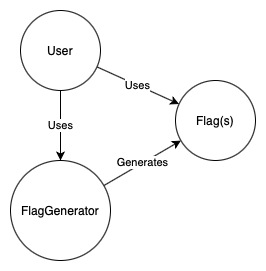
\includegraphics[width=0.5\textwidth]{FRs_WorkContext_Old.png}
    \caption{\textcolor{red}{[Old]} Context Diagram for FlagGenerator.}
    \label{fig:FRs_WC_O}
\end{figure}

\begin{figure}[h!]
    \centering
    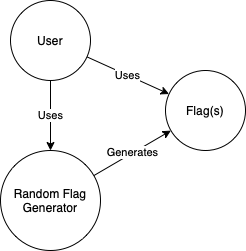
\includegraphics[width=0.5\textwidth]{FRs_WorkContext_New.png}
    \caption{\textcolor{red}{[New]} Context Diagram for the Random Flag Generator.}
    \label{fig:FRs_WC_N}
\end{figure}

\noindent \textcolor{red}{The Random Flag Generator (RFG) \sout{FlagGenerator}} is a standalone application that does not interact with other systems to operate. It consists of one actor, which is the user.

%\pagebreak

\subsubsection{Work Partitioning}

\begin{table}[h!]
    \centering
    \caption{Work Partitioning Events}
    \begin{tabularx}{\textwidth}{|c|X|X|X|}
        \hhline{|-|-|-|-|}
        \textbf{Event Number} & \textbf{Event Name} & \textbf{Input} & \textbf{Output} \\
        \hhline{|-|-|-|-|}
        1 & Entering the main menu & Keyboard/Mouse & Main Menu, \textcolor{red}{Start, Gallery, Settings and Help Menu Buttons \sout{Input String Field}} \\
        \hhline{|-|-|-|-|}
        \textcolor{red}{2} & \textcolor{red}{Entering the start menu} & \textcolor{red}{Mouse} & \textcolor{red}{Start Menu, Input String Field, Generate, Display, Back and Clear Buttons} \\
        \hhline{|-|-|-|-|}
        \textcolor{red}{3 \sout{2}} & Entering a new input string & Keyboard/Mouse & \textcolor{red}{\sout{Prompt}} \\
        \hhline{|-|-|-|-|}
        \textcolor{red}{4 \sout{3}} & Generating a new flag & \textcolor{red}{\sout{Keyboard/}}Mouse & Generated Flag \\
        \hhline{|-|-|-|-|}
        \textcolor{red}{5} & \textcolor{red}{Viewing a generated flag} & \textcolor{red}{Mouse} & \textcolor{red}{Generated Flag View} \\
        \hhline{|-|-|-|-|}
        \textcolor{red}{6} & \textcolor{red}{Closing a generated flag} & \textcolor{red}{Mouse} & \textcolor{red}{Previous Menu} \\
        \hhline{|-|-|-|-|}
        \textcolor{red}{7 \sout{4}} & Reading the instructions & \textcolor{red}{\sout{Keyboard/}}Mouse & Instructions \\
        \hhline{|-|-|-|-|}
        \textcolor{red}{8 \sout{5}} & Opening the settings menu & \textcolor{red}{\sout{Keyboard/}}Mouse & \textcolor{red}{Various \sout{Different}} Flag Generation Settings \\
        \hhline{|-|-|-|-|}
        \textcolor{red}{9} & \textcolor{red}{Changing the settings} & \textcolor{red}{Mouse} & \textcolor{red}{Changed Flag Generation Settings} \\
        \hhline{|-|-|-|-|}
        \textcolor{red}{10 \sout{6}} & Viewing the gallery & \textcolor{red}{\sout{Keyboard/}}Mouse & Generated Flags Gallery \\
        \hhline{|-|-|-|-|}
    \end{tabularx}
\end{table}

\begin{table}[h!]
    \centering
    \caption{Work Partitioning Summaries}
    \begin{tabularx}{\textwidth}{|c|X|}
        \hhline{|-|-|}
        \textbf{Event Number} & \textbf{Summary} \\
        \hhline{|-|-|}
        1 & The user, through the keyboard or mouse input, enters and is shown the main menu and \textcolor{red}{start, gallery, settings and help menu buttons \sout{input string field}}. \\
        \hhline{|-|-|}
        \textcolor{red}{2} & \textcolor{red}{The user, through mouse input, enters and is shown the start menu, input string field and generate, display, back and clear buttons}. \\
        \hhline{|-|-|}
        \textcolor{red}{3 \sout{2}} & The user, through the keyboard or mouse input, enters a string \textcolor{red}{into the input string field \sout{and is shown a prompt to begin flag generation}}. \\
        \hhline{|-|-|}
        \textcolor{red}{4 \sout{3}} & The user, through \textcolor{red}{\sout{the keyboard or}} mouse input, starts the flag generation. \textcolor{red}{\sout{After the flag generation has been completed, the user will be shown the generated flag.}} \\
        \hhline{|-|-|}
        \textcolor{red}{5} & \textcolor{red}{The user, through mouse input, opens the generated flag display view and is shown the generated flag.} \\
        \hhline{|-|-|}
        \textcolor{red}{6} & \textcolor{red}{The user, through mouse input, closes the generated flag display view and returns to the previous menu.} \\
        \hhline{|-|-|}
        \textcolor{red}{7 \sout{4}} & The user, \textcolor{red}{\sout{through keyboard or}} mouse input, chooses to read the instructions \textcolor{red}{on \sout{of}} using the \textcolor{red}{Random Flag Generator \sout{FlagGenerator}}. \\
        \hhline{|-|-|}
        \textcolor{red}{8} & \textcolor{red}{The user, through mouse input, opens the settings menu and is shown the various flag generation settings.} \\
        \hhline{|-|-|}
        \textcolor{red}{9 \sout{5}} & Before/after flag generation, the user can use \textcolor{red}{\sout{keyboard or}} mouse input to \textcolor{red}{change certain flag generation settings while in \sout{open}} the settings menu. After the settings have been changed, the user can (re)generate a flag with the updated settings taking effect. \\
        \hhline{|-|-|}
        \textcolor{red}{10 \sout{6}} & The user, though \textcolor{red}{\sout{the keyboard or}} mouse input, views their own gallery of current (and previously) generated flags. \\
        \hhline{|-|-|}
    \end{tabularx}
\end{table}

\pagebreak

\subsubsection{Individual Product Use Cases}

\begin{figure}[h!]
    \centering
    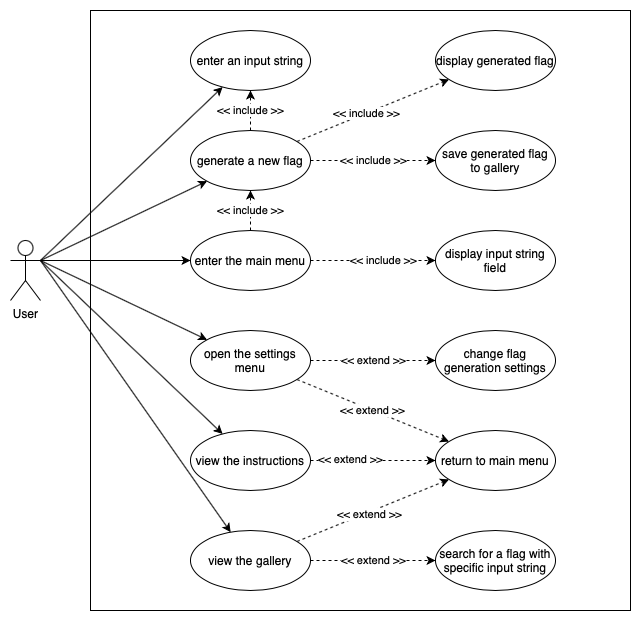
\includegraphics[width=0.75\textwidth]{FRs_UseCaseDiagram.png}
    \caption{Use Case Diagram that displays the main functionalities of the application.}
    \label{fig:FRs_UCD}
\end{figure}

\noindent The \textcolor{red}{below \sout{above}} use case diagram shows the various ways a user can interaction with our application. Generating a flag involves entering in an input string, which is an included use case. The other uses cases such as view instructions, open settings menu and view gallery are self-explanatory.

\pagebreak

\subsection{Functional Requirements}

\begin{enumerate}[label=BE\arabic*.]
    \begin{item}
        The \textbf{user} enters the main menu.
        \begin{enumerate}[label=FR\arabic*., series=frs]
            \item The \textbf{system} must present the \textbf{user} with the \textbf{main menu} and \textbf{input string field} for taking strings to generate flags from upon initializing the \textbf{GUI display}.
            
            \item The \textbf{system} must present the \textbf{buttons} to pull up the \textbf{instructions}, \textbf{flag gallery} and \textbf{settings menus}, or respond to the appropriate keyboard strokes.

            \item The \textbf{system} must allow the \textbf{user} to (re)enter in an input string into the \textbf{input string field} displayed on the \textbf{GUI}.

            \item The \textbf{system} must present the \textbf{user} with a \textbf{button} to enter in their input string and \textbf{start} the flag generation.

            \item The \textbf{system} must \textbf{present} the generated \textbf{flag} to the \textbf{user} in the main menu once it has finished being generated.

            \item The \textbf{system} must allow the \textbf{user} to \textbf{rerun} the flag generation after \textbf{settings} have been changed and \textbf{generate} a new flag that incorporates the changes to the settings.

            \item The \textbf{system} must \textbf{save} each generated \textbf{flag} to the user’s personal \textbf{gallery}, using the \textbf{input string} as its (default) name, adding numbers as needed.
        \end{enumerate}
    \end{item}

    \begin{item}
        The \textbf{user} enters in a new \textbf{input string}.
        \begin{enumerate}[label=FR\arabic*., resume*=frs]
            \item The \textbf{system} must present the \textbf{user} with a \textbf{button} to enter in their input string and \textbf{start} the flag generation.
        \end{enumerate}
    \end{item}

    \begin{item}
        The \textbf{user} starts the generation of a new \textbf{flag}.
        \begin{enumerate}[label=FR\arabic*., resume*=frs]
            \item The \textbf{system} must present the generated \textbf{flag} to the \textbf{user} in the main menu once it has finished being generated.

            \item The \textbf{system} must allow the \textbf{user} to \textbf{rerun} the flag generation after \textbf{settings} have been changed and \textbf{generate} a new flag that incorporates the changes to the settings.

            \item The \textbf{system} must \textbf{save} each generated \textbf{flag} to the user’s personal \textbf{gallery}, using the \textbf{input string} as its (default) name, adding numbers as needed.
        \end{enumerate}
    \end{item}

    \begin{item}
        The \textbf{user} reads the \textbf{instructions} for using FlagGenerator.
        \begin{enumerate}[label=FR\arabic*., resume*=frs]
            \item The \textbf{system} must provide instructions to the \textbf{user} on how to use the \textbf{flag generator}.

            \item The \textbf{system} must provide a way for the \textbf{user} to return to the \textbf{main menu}.
        \end{enumerate}
    \end{item}

    \begin{item}
        The \textbf{user} opens the settings menu before/after generating a \textbf{flag}.
        \begin{enumerate}[label=FR\arabic*., resume*=frs]
            \item The \textbf{system} must allow the \textbf{user} to change the \textbf{flag generator} settings.

            \item The \textbf{system} must specify the version of the \textbf{flag generator}.

            \item The \textbf{system} must provide a way for the \textbf{user} to return to the \textbf{main menu}.
        \end{enumerate}
    \end{item}

    \begin{item}
        The \textbf{user} opens the gallery.
        \begin{enumerate}[label=FR\arabic*., resume*=frs]
            \item The \textbf{system} must present the \textbf{user} with a list of all \textbf{flags} and the \textbf{input string} used to generate them.

            \item \textcolor{red}{\sout{The \textbf{system} must allow the \textbf{user} to search for specific flags based on input string.}}

            \item The \textbf{system} must provide a way for the \textbf{user} to return to the \textbf{main menu}.
        \end{enumerate}
    \end{item}
\end{enumerate}

\section{Non-functional Requirements}

\subsection{Look and Feel Requirements}

\subsubsection{Appearance Requirements}
\begin{enumerate}[label=LF\arabic*., series=lfs]
    \item A simple, intutitive and non-cluttered UI must be used. \textcolor{red}{Fit criterion: All three developers of Random Flag Generator agree with this statement}
\end{enumerate}

\subsubsection{Style Requirements} 
\begin{enumerate}[label=LF\arabic*., resume=lfs]
    \item The program must generate high qu\textcolor{red}{a}lity images that are aesthetically pleasing. \textcolor{red}{Fit criterion: 90\% of all testers were satisfied with the flag quality}
    \item Picture colours must be within certain colour ranges. \textcolor{red}{Fit criterion: All three developers of Random Flag Generator agree with this statement}
    \item All image components must be visible in the generated image. \textcolor{red}{Fit criterion: All three developers of Random Flag Generator agree with this statement 80\% of the times with some similar colours being harder to differentiate.}
\end{enumerate}

\subsection{Usability and Humanity Requirements}
\subsubsection{Ease of Use Requirements}
\begin{enumerate}[label=UH\arabic*., series=uhs]
    \item UI components must be placed in a logically flowing manner. \textcolor{red}{Fit criterion: All three developers of Random Flag Generator agree with this statement}
    \item User must not have to jump between interfaces to accomplish a task. \textcolor{red}{Fit criterion: All three developers of Random Flag Generator agree with this statement}
    \item Program must be easy-to-use for people aged \textcolor{red}{$\hyperlink{min_age}{MIN\_AGE}$ \sout{7}} or older. \textcolor{red}{Fit criterion: 100\% testers of Random Flag Generator agree with this statement}
    \item \textcolor{red}{\sout{The program must use intuitive keyboard inputs to perform actions.}}
\end{enumerate}
                           
\subsubsection{Personalization Requirements}
\begin{enumerate}[label=UH\arabic*., resume=uhs]
    \item User must be able to select output specifications (type of hashing, type of image file, etc.). \textcolor{red}{Fit criterion: All three developers of Random Flag Generator agree with this statement}
    \item \textcolor{red}{\sout{User must be able to modify their image gallery (add, delete).}}
\end{enumerate} 
\subsubsection{Learning Requirements} 
\begin{enumerate}[label=UH\arabic*., resume=uhs]
    \item The user should be able to use the program with no prior experience. \textcolor{red}{Fit criterion: All three developers and testers of Random Flag Generator agree with this statement}
    \item The user must be able to access a brief instructions blurb. \textcolor{red}{Fit criterion: All testers of Random Flag Generator agree with this statement}
    \item The user must be able to use the program by following the main UI instructions only. \textcolor{red}{Fit criterion: All testers and three developers of Random Flag Generator agree with this statement}
\end{enumerate} 

\subsubsection{Understandability Requirements}
\begin{enumerate}[label=UH\arabic*., resume=uhs]
    \item The program must use consistent language throughout. \textcolor{red}{Fit criterion: All three developers of Random Flag Generator agree with this statement}
    \item The program must use simplified terminology wherever possible. \textcolor{red}{Fit criterion: All three developers of Random Flag Generator agree with this statement}
\end{enumerate}

\subsubsection{Accessibility Requirements}
\begin{enumerate}[label=UH\arabic*., resume=uhs]
    \item Program must use easy-to-read fonts and font sizes. \textcolor{red}{Fit criterion: 100\% of testers of Random Flag Generator agree with this statement}
    \item \textcolor{red}{\sout{Program must provide a color-blind friendly UI.}}
\end{enumerate}

\subsection{Performance Requirements}
\subsubsection{Speed Requirements}
\begin{enumerate}[label=PE\arabic*., series=pes]
    \item Program must minimize the time taken to generate an image. \textcolor{red}{Fit criterion: All three developers of Random Flag Generator agree with this statement}
    \item Program must minimize the time taken to process the downloading of an image. \textcolor{red}{Fit criterion: All three developers of Random Flag Generator agree with this statement}
    \item Program must minimize the time taken to load in a user's gallery. \textcolor{red}{Fit criterion: All three developers of Random Flag Generator agree with this statement}
\end{enumerate}

\subsubsection{Safety-Critical Requirements}
$N/A$
\subsubsection{Precision or Accuracy Requirements}
\begin{enumerate}[label=PE\arabic*., resume=pes]
    \item Different hashing systems must all deliver consistent and precise outputs. \textcolor{red}{Fit criterion: All three developers of Random Flag Generator agree with this statement}
    \item Generated images must have accurately placed components (matching templates). \textcolor{red}{Fit criterion: All three developers of Random Flag Generator agree with this statement}
    \item Colours in the generated image must be precise (the hexadecimal value). \textcolor{red}{Fit criterion: All three developers of Random Flag Generator agree with this statement}
\end{enumerate}

\subsubsection{Reliability and Availability Requirements}
\begin{enumerate}[label=PE\arabic*., resume=pes]
    \item The program must be available to run anytime in the day. \textcolor{red}{Fit criterion: All three developers of Random Flag Generator agree with this statement}
\end{enumerate}  

\subsubsection{Robustness or Fault-Tolerance Requirements}
$N/A$
\subsubsection{Capacity Requirements}
\begin{enumerate}[label=PE\arabic*., resume=pes]
    \item \textcolor{red}{\sout{User must be able to store up to a certain maximum number of generated images.}}
    \item The program must limit the number of users to one per machine. \textcolor{red}{Fit criterion: All three developers of Random Flag Generator agree with this statement}
\end{enumerate} 

\subsubsection{Scalability or Extensibility Requirements}
\begin{enumerate}[label=PE\arabic*., resume=pes]
    \item Program should allow for the addition of other hashing functions. \textcolor{red}{Fit criterion: All three developers of Random Flag Generator agree with this statement}
    \item Program should allow for the addition of other flag components. \textcolor{red}{Fit criterion: All three developers of Random Flag Generator agree with this statement}
\end{enumerate} 
\subsubsection{Longevity Requirements}
\begin{enumerate}[label=PE\arabic*., resume=pes]
    \item Program must be functional with exisiting software and hardware until Spring 2023. \textcolor{red}{Fit criterion: All three developers of Random Flag Generator agree with this statement}
\end{enumerate} 
\subsection{Operational and Environmental Requirements}
\subsubsection{Expected Physical Environment}
\begin{enumerate}[label=PE\arabic*., resume=pes]
    \item Program must not require an internet connection to function. \textcolor{red}{Fit criterion: All three developers of Random Flag Generator agree with this statement}
    \item Program must run on any computer that can support the Python language. \textcolor{red}{Fit criterion: All three developers of Random Flag Generator agree with this statement}
\end{enumerate} 

\subsection{Requirements for Interfacing with Adjacent Systems}
\begin{enumerate}[label=PE\arabic*., resume=pes]
    \item Program must not alter files outside the working directory. \textcolor{red}{Fit criterion: All three developers of Random Flag Generator agree with this statement}
\end{enumerate} 

\subsubsection{Productization Requirements}
\begin{enumerate}[label=PE\arabic*., resume=pes]
    \item Program must be distributed as an executable file. \textcolor{red}{Fit criterion: All three developers of Random Flag Generator agree with this statement}
\end{enumerate} 

\subsection{Release Requirements}
\begin{enumerate}[label=RR\arabic*., series=rrs]
    \item The program must be released on or by April 12, 2022. \textcolor{red}{Fit criterion: All three developers of Random Flag Generator agree with this statement}
\end{enumerate} 

\subsection{Maintainability and Support Requirements}

\subsubsection{Maintenance Requirements}
\begin{enumerate}[label=MA\arabic*., series=mas]
    \item Source code must be modularized with low cohesion. \textcolor{red}{Fit criterion: All three developers of Random Flag Generator agree with this statement}
    \item Source code must be fully commented. \textcolor{red}{Fit criterion: All three developers of Random Flag Generator agree with this statement}
    \item Full program documentation must be available. \textcolor{red}{Fit criterion: All three developers of Random Flag Generator agree with this statement}
    \item Proper and consistent coding style must be followed. \textcolor{red}{Fit criterion: All three developers of Random Flag Generator agree with this statement}
\end{enumerate} 
\subsubsection{Supportability Requirements}
\begin{enumerate}[label=MA\arabic*., resume=mas]
    \item The program's repository must be made public to allow for issue raising. \textcolor{red}{Fit criterion: All three developers of Random Flag Generator agree with this statement}
\end{enumerate}
\subsubsection{Adaptability Requirements}
\begin{enumerate}[label=MA\arabic*., resume=mas]
    \item This program must be able to be run on all major computer OS/platforms. \textcolor{red}{Fit criterion: All three developers of Random Flag Generator agree with this statement}
\end{enumerate}
\subsection{Security Requirements} 
\subsubsection{Access Requirements}
\begin{enumerate}[label=SR\arabic*., series=srs]
    \item User must only be able to modify their own gallery. \textcolor{red}{Fit criterion: All three developers of Random Flag Generator agree with this statement}
    \item User must only be able to generate flags for their gallery. \textcolor{red}{Fit criterion: All three developers of Random Flag Generator agree with this statement}
\end{enumerate}
\subsubsection{Integrity Requirements}
\begin{enumerate}[label=SR\arabic*., resume=srs]
    \item User must be able modify their saved flag images (gallery). \textcolor{red}{Fit criterion: All three developers of Random Flag Generator agree with this statement}
    \item In general, the input string must not be able to be deciphered from a generated image. \textcolor{red}{Fit criterion: All three developers of Random Flag Generator agree with this statement}
\end{enumerate}

\subsubsection{Privacy Requirements}
\begin{enumerate}[label=SR\arabic*., resume=srs]
    \item A user's gallery must not be visible to other users. \textcolor{red}{Fit criterion: All three developers of Random Flag Generator agree with this statement}
    \item User inputted strings must be deleted after image generation. \textcolor{red}{Fit criterion: All three developers of Random Flag Generator agree with this statement}
\end{enumerate}
\subsubsection{Audit Requirements}
$N/A$
\subsubsection{Immunity Requirements}
\begin{enumerate}[label=SR\arabic*., resume=srs]
    \item Program must not have any obvious vulnerabilties. \textcolor{red}{Fit criterion: All three developers of Random Flag Generator agree with this statement}
\end{enumerate}

\subsection{Cultural Requirements}
\subsubsection{Cultural Requirements}
\begin{enumerate}[label=CP\arabic*., series=cps]
    \item Flag components must be respectful of countries' cultures. \textcolor{red}{Fit criterion: All three developers of Random Flag Generator agree with this statement}
    \item Offensive flag components must not be included in possible flag components. \textcolor{red}{Fit criterion: All three developers of Random Flag Generator agree with this statement}
    \item Input strings must have only valid hashable characters. \textcolor{red}{Fit criterion: All three developers of Random Flag Generator agree with this statement}
\end{enumerate}
\subsubsection{Political Requirements}
\begin{enumerate}[label=CP\arabic*., resume=cps]
    \item No flag generated should promote any one political belief. \textcolor{red}{Fit criterion: All three developers of Random Flag Generator agree with this statement}
    \item No flag generated should offend one's political views. \textcolor{red}{Fit criterion: All three developers of Random Flag Generator agree with this statement}
\end{enumerate}

\subsection{Legal Requirements}
\subsubsection{Compliance Requirements}
\begin{enumerate}[label=LR\arabic*., series=lrs]
    \item Source code must follow the license under which it was obtained. \textcolor{red}{Fit criterion: All three developers of Random Flag Generator agree with this statement}
    \item Personal information must be kept secure and local to the user. \textcolor{red}{Fit criterion: All three developers of Random Flag Generator agree with this statement}
\end{enumerate}
\subsubsection{Standards Requirements}
$N/A$
\subsection{Health and Safety Requirements}
$N/A$\\
This section is not in the original Volere template, but health and safety are
issues that should be considered for every engineering project.

\section{Project Issues}

\subsection{Open Issues}

None have been documented so far, and there are no open issues on PAGAN's repository at the time of this SRS. 

\subsection{Off-the-Shelf Solutions}

There are similar products available, such as Scrontch's Flag Designer https://flag-designer.appspot.com/ and other flag generators; however, they do not take in an input string and they do not give users the option to personalize their flag. There are also existing products that use strings and hashing algorithms to generate random images, but not flags.

\subsection{New Problems}

Some problems that may exist after this software is launched include \textcolor{red}{lower} flag image quality, issues of copyright, and inappropriate use of flags. Users will be able to have high resolution images, but they may have a lower resolution flag than expected.

\subsection{Tasks}

Project tasks are scheduled and assigned. Please refer to project Gantt chart: ../ProjectSchedule/3XA3Ganttchart.pdf

\subsection{Migration to the New Product}

Since the software is simple and discrete, there is no need for migration to the new product. The gallery within the application will allow data to be stored.

\subsection{Risks}

This project has minimal risk because it is intended to be user-friendly and simple. There is, however, a risk of poor performance and unexpected application crashes. This is be minimized with intensive testing. There are also risks of low team productivity; however, this will be managed through our communication and problem solving skills.

\subsection{Costs}

There is no monetary cost for this project, as it will be developed as an open source software. The cost of time and effort are to be considered. This project is within the scope of the SFWRENG 3XA3 course. Therefore, the resource cost will be reasonable.

\subsection{User Documentation and Training}

\subsubsection{Documentation}

Software instructions will be included in a display window that is easily accessible from the main menu, for users to understand how to use the product along with its features.

\subsubsection{Training}

No training is required to use this application. 

\subsection{Waiting Room}

Some features that may be added in later releases include:

\begin{enumerate}
    \item Better resolutions and a \textcolor{red}{better} GUI
    \item Different language settings
    \item Sharing options through social media
    \item \textcolor{red}{Able to save images in different formats}
    \item \textcolor{red}{Online version}
    \item \textcolor{red}{More settings options}
\end{enumerate}

\subsection{Ideas for Solutions}

N/A

\bibliographystyle{plainnat}

\bibliography{SRS}

\newpage

\section{Appendix}

This section has been added to the Volere template.  This is where you can place
additional information.

\subsection{Symbolic Parameters}

The definition of the requirements will likely call for SYMBOLIC\_CONSTANTS.
Their values are defined in this section for easy maintenance. \\ \\
\textcolor{red}{$\hypertarget{min_age}{MIN\_AGE}$ = 7} \\

\end{document}